%%%%%%%%%%%%%%%%%%%%%%%%%%%%%%%%%%%%%%%%%%%%%%%%%%%%%%%%%%%%%%%%%%%%%%%%%%%%%%%
% Titel:   Anhang
% Autor:   Nicola K�ser
%%%%%%%%%%%%%%%%%%%%%%%%%%%%%%%%%%%%%%%%%%%%%%%%%%%%%%%%%%%%%%%%%%%%%%%%%%%%%%%
% Umschalten der Seitennummerierung auf (Kapitelbuchstabe)-(Seite, 0-indexiert)
\newcommand{\mypagenumbering}{
	% Seitenzahl umschalten auf eigene Nummerierung: A-1, A-2, ...
	\renewcommand{\thepage}{\Alph{chapter}-\arabic{page}}
	% Seitenz�hler auf 0, damit die Seite 1 des Anhangs dann auch A-1
	\setcounter{page}{0}
}
%
% Anhang A
\chapter{Testprotokoll}\label{ch:anhang_a}
\mypagenumbering
\todo{PDF erstellen und includen}%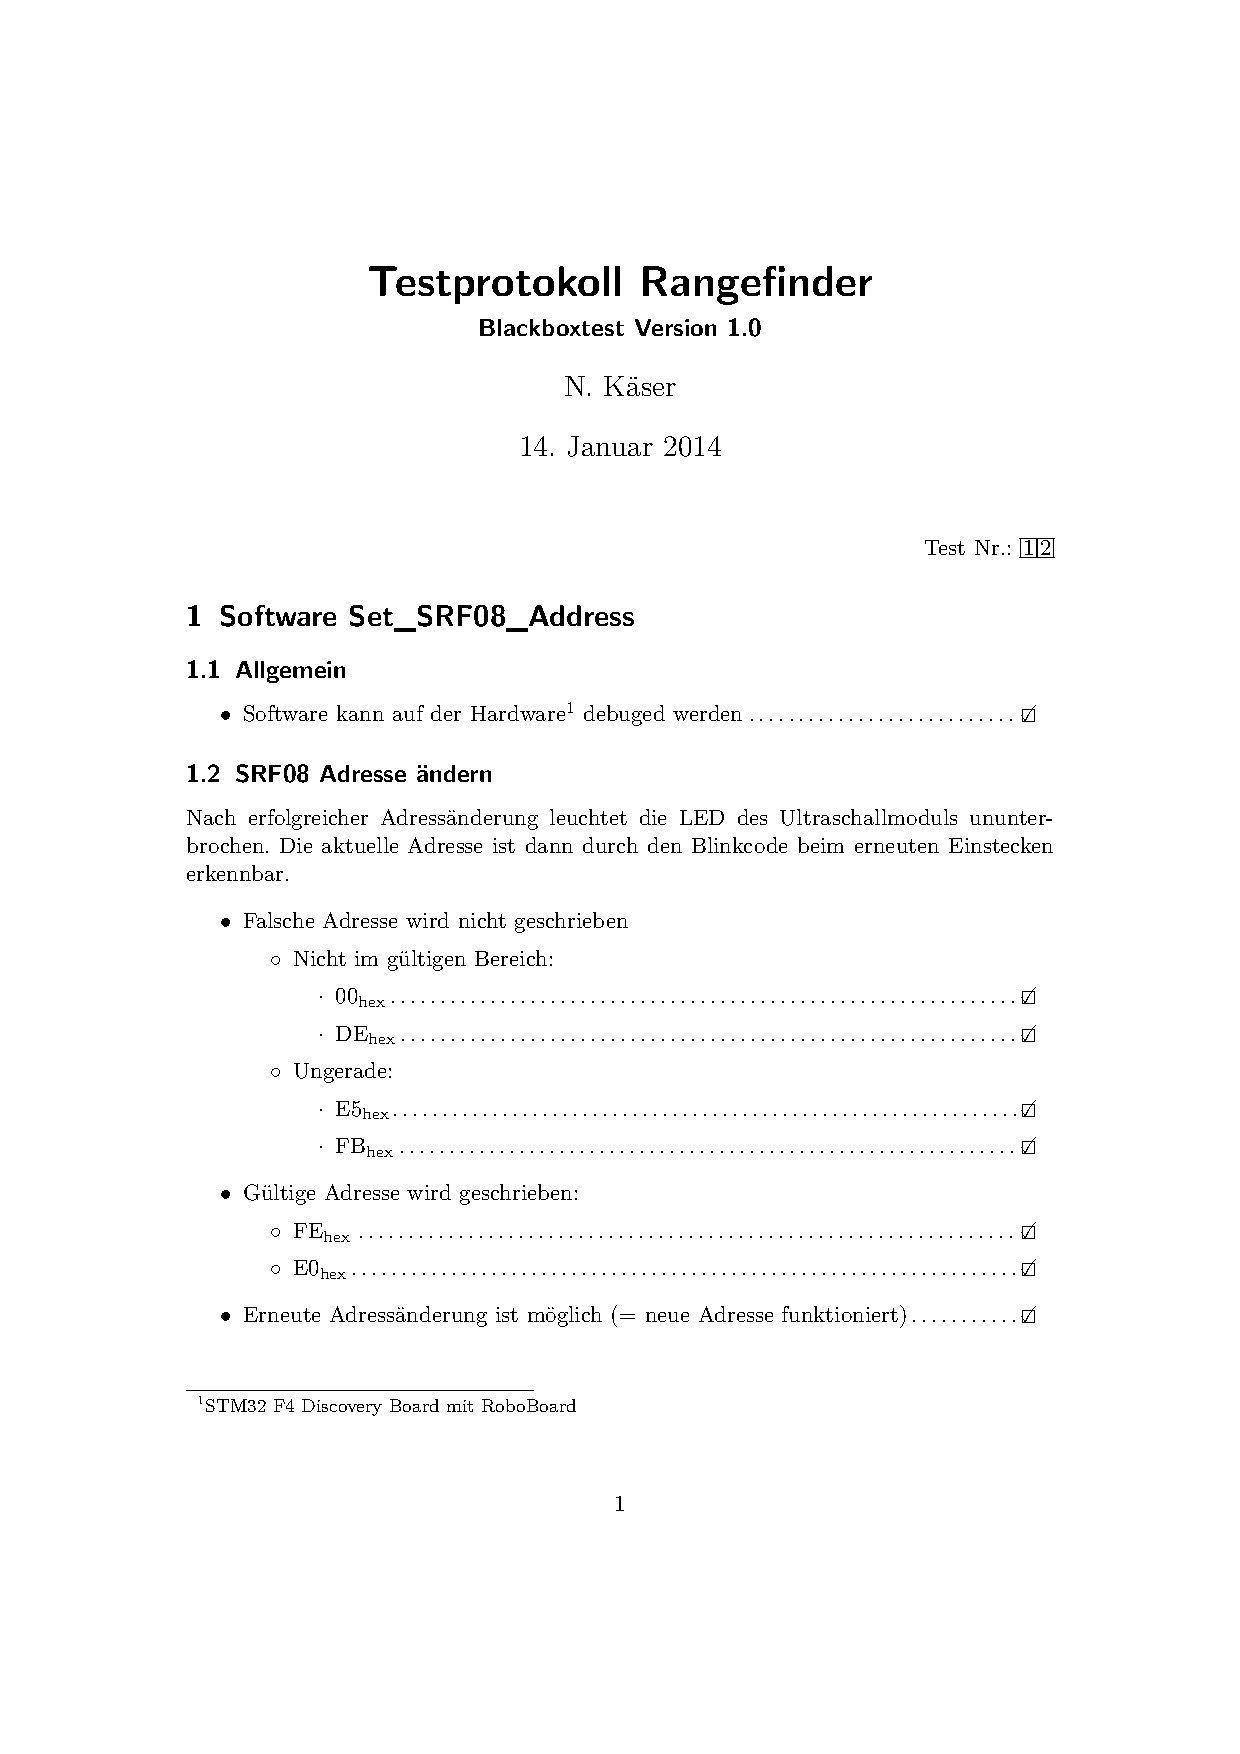
\includepdf[scale=1,pages=-]{appendix/anhangB_Testprotokoll}